\documentclass[handout]%
{beamer}
%\usetheme{Execushares}
\usetheme{AnnArbor}
\usecolortheme{beaver}
%\setbeamercolor{title}{parent=structure,bg=green!50!black,fg=white}
%\usecolortheme{dolphin}
\setbeamertemplate{navigation symbols}{}%remove navigation symbols

\usepackage{amsmath}
\usepackage{amssymb}
\usepackage{amsthm}
%\usepackage[utf8]{inputenc}
\usepackage[czech]{babel}
\usepackage{tikz-cd}
\usepackage[mathscr]{euscript}
\usepackage[IL2]{fontenc}
\usepackage{mathtools}
\usepackage[normalem]{ulem}

%\usetikzlibrary{calc,shapes.callouts,shapes.arrows}

%\usepackage{beamerarticle}

%\usepackage{bbm}

\def\rllap#1{\hbox to0pt{\hss#1\hss}}

%\newcommand{\bubblethis}[2]{
        %\tikz[remember picture,baseline]{\node[anchor=base,inner sep=0,outer sep=0]%
        %(#1) {\underline{#1}};\node[overlay,cloud callout,callout relative pointer={(-0.2cm,+0.7cm)},%
        %aspect=2.5,fill=yellow!90] at ($(#1.north)+(-0.5cm,1.6cm)$) {#2};}%
    %}%
		%
%\newcommand{\speechthis}[2]{
        %\tikz[remember picture,baseline]{\node[anchor=base,inner sep=0,outer sep=0]%
        %(pom) {#1};\node[overlay,ellipse callout,fill=blue!50] 
        %at ($(pom.north)+(1cm,+0.8cm)$) {#2};}%
    %}%
		
\newcommand{\R}{\mathbb R}
\def\d{\text{d}}

%\title{Limity funkcí}
\author{Alexander Slávik} %  and J. Trlifaj
\title{Derivace funkce}
\subtitle{Monotonie a extrémy}
\institute{Gymnázium Voděradská}
\date{27. 1. 2021}

\begin{document}


\section{Monotonie funkcí}

\begin{frame}
	\frametitle{Monotónní funkce a derivace}
	Monotónní funkce = rostoucí, klesajcí, neklesající, nerostoucí\dots \pause
	\begin{block}{Věta}
	Nechť funkce $f$ má v každém bodě intervalu $(a, b)$ derivaci, která je navíc ve všech bodech onoho intervalu kladná / záporná / nezáporná / nekladná.
	Pak je $f$ na tomto intervalu rostoucí / klesající / neklesající / nerostoucí.
	
	\smallskip\pause
	Je-li $f$ definovaná a spojitá i v bodech $a$ nebo $b$ nebo obou, pak závěr platí i pro intervaly $\langle a; b)$ nebo $(a; b\rangle$ nebo $\langle a; b\rangle$.
	\end{block}
	\pause
	Funkce může být na nějakém intervalu např. rostoucí a přitom tam mít nulovou derivaci; např $f(x) = x^3$:
	\vskip-5mm
	\[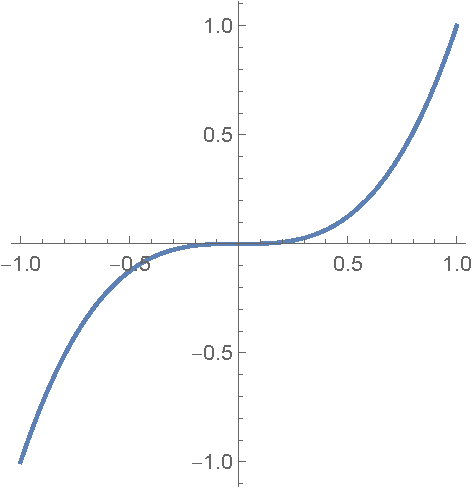
\includegraphics[height=.3\vsize]{grafy/cube.pdf}\]
\end{frame}


\begin{frame}
	\frametitle{Použití}
	\begin{itemize}
		\item \uv{Typicky} půjde definiční obor $f$ rozdělit na intervaly, ve kterých bude funkce rostoucí či klesající.\pause
		\item To zjistíme tak, že zjišťujeme znaménko derivace.
	\end{itemize}
\end{frame}



\section{Extrémy funkcí}

\begin{frame}
	\frametitle{Klíčová věta o extrémech}
	\begin{block}{Věta}
	Má-li funkce $f$ v bodě $x_0 \in \R$ (neostré) lokální maximum či minimum a existuje-li derivace $f'(x_0)$, potom $f'(x_0) = 0$.
	\end{block}
	
	\pause
	\[ 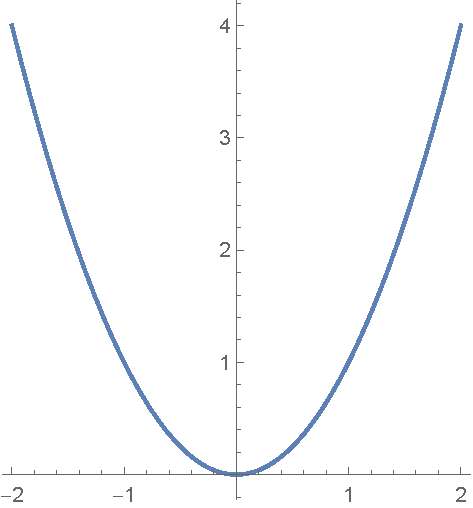
\includegraphics[height=.4\vsize]{grafy/kvadr.pdf} \]
	Např. funkce $f(x) = x^2$ má v nule minimum a derivace tam existuje; \pause vskutku tedy $f'(0) = 2 \cdot 0 = 0$.	
\end{frame}

\begin{frame}
\frametitle{Co NEplatí I}
	\begin{alertblock}{Neplatí!}
		Funkce má v $x_0$ lokální extrém $\Rightarrow$ má tam nulovou derivaci.
	\end{alertblock}
	\pause
	$f(x) = |x|$ má v nule minimum, ovšem derivace tam vůbec neexistuje.\[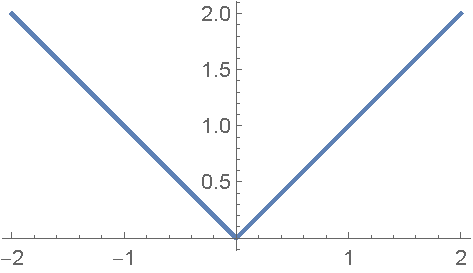
\includegraphics[height=.4\vsize]{grafy/abs.pdf}\]
	
\end{frame}


\begin{frame}
\frametitle{Co NEplatí II}

	\begin{alertblock}{Neplatí!}
		Funkce má v $x_0$ nulovou derivaci $\Rightarrow$ má tam lokální extrém.
	\end{alertblock}
	\pause
	$f(x) = x^3$ má v nule nulovou derivaci, ovšem není tam minimum ani maximum.\[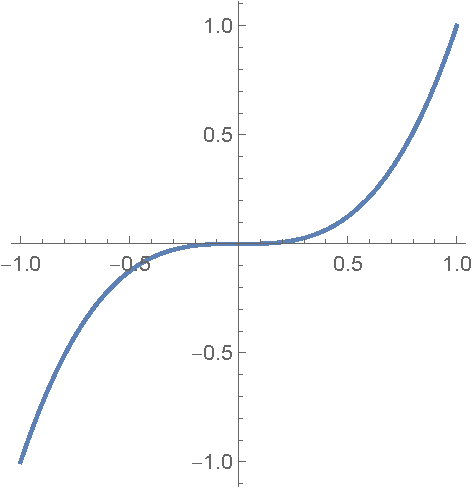
\includegraphics[height=.4\vsize]{grafy/cube.pdf}\]
\end{frame}


\begin{frame}
\frametitle{Typické použití}
	Máme nějakou funkci $f$.\pause
	\begin{enumerate}
		\item Spočteme její derivaci.\pause
		\item Nalezneme nulové body derivace, tzv. \alert{stacionární body} či též \alert{body podezřelé z extrému} \pause (řešíme rovnici $f'(x) = 0$).\pause
		\item Rozhodneme, které z těchto bodů jsou opravdu extrémy a jaké extrémy to jsou.\pause
		\item (Nějak naložíme s body, ve který derivace neexistuje.)
	\end{enumerate}
\end{frame}


\begin{frame}
\frametitle{Jak poznat extrémy}
	Jak poznat, které ze stacionárních bodů (tj. nulových bodů derivace) jsou opravdu extrémy?\pause
	\begin{block}{Věta}
	Pokud
	\begin{itemize}
		\item existuje derivace funkce $f$ na nějakém okolí bodu $x_0 \in \R$,\pause
		\item je $f'(x_0) = 0$,\pause
		\item v $x_0$ derivace \alert{\uv{mění znaménko}}, tj. na nějakém prstencovém pravém okolí je derivace jen kladná a na nějakém prstencovém levém okolí je jen záporná (nebo naopak),\pause
	\end{itemize}
	tak má $f$ v $x_0$ lokální extrém; \pause je to lokální maximum, pokud je derivace \alert{vlevo kladná a vpravo záporná}, a lokální minimum, pokud je \alert{vlevo záporná a vpravo kladná}.
	\end{block}
\end{frame}


\end{document}
